\chapter{Opis techniczny benchmarku}
\section{Streszczenie}
Załącznik ten jest przeznaczony dla osób, które w przyszłości chciałyby rozszerzać,
rozbudowywać omawiany system np.: studentów kolejnych roczników. Jego celem jest zatem dostarczenie
możliwie jak największej porcji użytecznych informacji dla takich osób.

Omawiany w tej pracy benchmark powstawał na zasadzie prototypowania i określania przyrostów funkcjonalnych,
gdyż nie można było już na samym początku prac, przewidzieć dokładnie 
jego architektury. Na taki stan rzeczy złożyło się kilka faktów:
\begin{itemize}
\item Autor benchmarku w momencie rozpoczynania prac nie posiadał doświadczenia związanego z budową tego typu
rozwiązań, w związku z czym nie był w stanie przewidzieć wszystkich problemów jakie na jego drodze mogły się
pojawić.
\item Budowane rozwiązanie nie posiadało innego adekwatnego pierwowzoru, na którym można było by się w pełni oprzeć.
Wspomniany w rozdziale \ref{chap:teo} benchmark TPC-C pod wieloma względami różnił się od planowanego systemu.
\end{itemize}
Przyjęcie tego typu strategii jest bardzo często stosowane podczas budowy rozwiązań eksperymentalnych, 
w których trudno jest przewidzieć do końca architekturę. Poza stworzeniem systemu, równorzędnym celem 
było zdobycie doświadczenia i wyciągnięcie wniosków odnośnie przyjętych założeń projektowych.

W przypadku pytań/uwag do niniejszej pracy autor oferuje swoją pomoc. W tym celu należy kontaktować się 
poprzez adres email: mirek.begier@gmail.com.

\section{Fizyczna struktura systemu}
Omawiane rozwiązanie zostało wykonane w oparciu o środowisko Eclipse w wersji 3.2.
System składa się z 4 projektów:
\begin{itemize}
\item JXmlSerializer -- jest to projekt biblioteki dostępu do plików xml poprzez stosowanie adnotacji klas.
Klasy takie są następnie serializowane i deserialiozwane do formatu xml. Idea tej biblioteki została zaczerpnięta
ze środowiska .Net~\cite{.Net1}~\cite{.NetXmlSerializer1}, w którym istnieje podobny mechanizm oparty o atrybuty. 
W stworzonym benchmarku biblioteka została wykorzystana w celu uproszczenia odczytywania i zapisywania plików xml reprezentujących:
\begin{itemize}
\item model bazy danych -- pakiet org.jdbmeasure.model.database,
\item model obciążenia bazy danych -- pakiet org.jdbmeasure.model.load,
\item model testu -- pakiet org.jdbmeasure.model.test,
\item plik konfiguracyjny klienta RTE -- pakiet org.jdbmeasure.rte.config.
\end{itemize}
Dla każdego z tych plików istnieją klasy z adnotacjami, stąd w powyższym wyliczeniu występują po myślniku nazwy pakietów,
zawierających te klasy. Bliższy opis biblioteki JXmlSerializer znajduje się dalej.%punkcie \ref{xmlser}.
\item JDBMeasure -- projekt ten zawiera klasy i pakiety stanowiące korzeń systemu. Bliższy opis znajduje się w dalszej części pracy.
\item JDBMeasureRCP -- projekt ten zawiera klasy i pakiety dotyczące interfejsu graficznego serwera benchmarku. Projekt ten
jest projektem aplikacji serwera, zgodnej z architekturą Eclipse RCP. Znajdują się tutaj zatem:
\begin{itemize}
\item widoki,
\item edytory,
\item okna dialogowe,
\item kreatory.
\end{itemize}
Projekt ten korzysta z klas zawartych w projekcie JDBMeasure, jego głównym zadaniem jest wizualizacja zawartych tam mechanizmów benchmarku.
\item JDBMeasureRCPExtJars -- jest projektem specyficznym dla aplikacji Eclipse RCP, zawiera on wszystkie biblioteki zewnętrzne dla tego typu aplikacji.
Znajdują się tutaj zatem wyłącznie pliki jar bibliotek takich jak:
\begin{itemize}
\item Hibernate 3.1~\cite{Hibernate1},
\item Hibernate Annotation 3.1~\cite{HibernateAnn1},
\item Spring 2.0~\cite{Spring1},
\item JFreeChart 1.0.1~\cite{JFreeChart1}.
\end{itemize} 
Umieszczenie plików jar w osobnym projekcie jest niezbędne ze względu na mechanizmy bezpieczeństwa i hierarchię ClassLoader'ów
aplikacji RCP.
\end{itemize}

\section{JXmlSerializer -- opis biblioteki}%\label{xmlser}
JXmlSerializer jest narzędziem do serializacji i deserializacji obiektów do formatu xml,
biblioteka ta powstała niezależnie od budowanego benchmarku, w celu ułatwienia pracy z dokumentami xml.
Główna klasa biblioteki używa adnotacji do tworzenia mapowań obiektów na dokumenty xml.
Poniżej zamieszczono przykładową klasę wraz z mapowaniami jej pól do dokumentu xml. 
\begin{quote}
\begin{Verbatim}
@XmlRoot("person")
public class Person {
	private String firstname;
	private String surname;
	private String description;
	private Sex sex;

	@XmlAttribute("firstname")
	public String getFirstname() {
		return this.firstname;
	}
	public void setFirstname(String firstname) {
		this.firstname = firstname;
	}

	@XmlAttribute("surname")
	public String getSurname() {
		return this.surname;
	}
	public void setSurname(String surname) {
		this.surname = surname;
	}

	@XmlElement("description")
	public String getDescription() {
		return description;
	}
	public void setDescription(String description) {
		this.description = description;
	}
	
	@XmlAttribute("sex")
	public Sex getSex() {
		return sex;
	}
	public void setSex(Sex sex) {
		this.sex = sex;
	}
}
\end{Verbatim}
\end{quote}
A zatem jedyne co należy zrobić by móc używać tej biblioteki, jest użycie we własnej klasie adnotacji 
z pakietu org.jxmlserializer.annotations, a następnie można już bardzo łatwo serializować obiekty:
\begin{quote}
\begin{Verbatim}
JXmlSerializer<Person> serializer 
	= new JXmlSerializer<Person>(Person.class);
serializer.serialize(file, person);
\end{Verbatim}
\end{quote}
oraz je deserializować z dokumentów xml:
\begin{quote}
\begin{Verbatim}
JXmlSerializer<Person> serializer 
	= new JXmlSerializer<Person>(Person.class);
Person person = serializer.deserialize(file);
\end{Verbatim}
\end{quote}
Powyższe informacje są wystarczające do zrozumienia kontekstu zastosowania biblioteki w omawianym benchmarku.
Głównym powodem wydzielenia kodu tej biblioteki, jako oddzielnego projektu, była jej uniwersalność -- biblioteka ta
może znaleźć zastosowanie wszędzie tam, gdzie pracuje się z dokumentami xml.

\section{JDBMeasure - omówienie projektu}
Jak już wspomniano JDBMeasure jest głównym projektem benchmarku, skupia on bowiem wszystkie te klasy,
które wykonują kod związany z główną funkcjonalnością aplikacji. Struktura tego projektu składa się 
z następujących katalogów:
\begin{quote}
\begin{Verbatim}
<DIR>          bin -- katalog skompilowanych klas,
   5 538 build.xml -- plik projektu anta,
<DIR>          doc -- katalog zawierający dokumentację, 
<DIR>          etc -- szablony i  dodatki,
<DIR>          ftp -- kod źródłowy serwera ftp,
<DIR>          lib -- wymagane biblioteki,
<DIR>          src -- kody źródłowe klas,
<DIR>          test -- kody źródłowe testów jednostkowych.
\end{Verbatim}
\end{quote}
Katalog doc zawiera ogólnie rozumianą dokumentację:
\begin{itemize}
\item JavaDoc kodu źródłowego -- podkatalog /doc/javadoc,
\item prezentacje benchmarku przygotowywane w ramach seminarium dyplomowego -- podkatalog /doc/presentations,
\item opis XmlSchema dla modeli -- podkatalog /doc/xmlschemas,
\item notatki -- podkatalog /doc/notes,
\item oraz pracę magisterską w LaTex'u -- podkatalog /doc/mgr/desc.
\end{itemize}
Nie mniej jednak najważniejsze w tym projekcie są kody źródłowe klas z katalogu src. 
Struktura pakietów przedstawia się następująco:
\begin{quote}
\begin{Verbatim}
\---org
    \---jdbmeasure
        +---database
        |   \---generator
        |       \---column
        |           \---exception
        +---model
        |   +---database
        |   |   \---classbuilder
        |   +---load
        |   \---test
        +---rte
        |   +---config
        |   +---info
        |   \---test
        |       \---properties
        +---server
        |   +---config
        |   \---info
        +---test
        |   +---datasource
        |   +---result
        |   \---script
        |       +---generator
        |       \---metadata
        \---util
            +---beans
            +---file
            +---math
            \---net\end{Verbatim}
\end{quote}
W dalszej części tego punktu zostaną omówione poszczególne pakiety
\subsection{Pakiet org.jdbmeasure.database}
Pakiet org.jdbmeasure.database zawiera klasy wykorzystywane podczas tworzenia populacji bazy danych,
jak i skryptów testowych. Większość klas tego pakietu służy do generowania danych poszczególnych kolumn, rekordów czy relacji.
Na rys.~\ref{rys:uml01} przedstawiono uproszczony diagram klas tego pakietu.
\begin{figure}[h]
\begin{center}
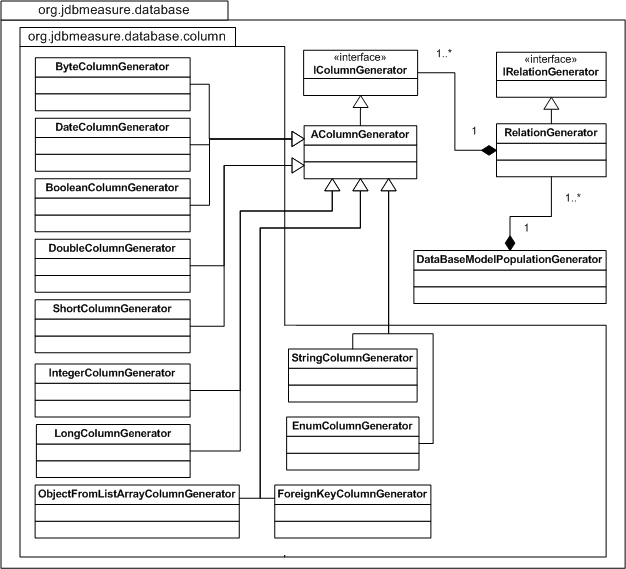
\includegraphics[width=1.0\linewidth]{figures/uml01.png}%[width=0.9\linewidth]
\end{center}
\caption{Diagram klas pakietu org.jdbmeasure.database}\label{rys:uml01}
\end{figure}
Klasa DataBaseModelPopulationGenerator jest odpowiedzialna za tworzenie populacji bazy danych. Znaczną część tego pakietu
stanowią klasy implementujące interfejs IColumnGenerator, są to klasy generatorów kolumn różnego typu wartości. 

\subsection{Pakiet org.jdbmeasure.model}
Pakiet ten zawiera klasy reprezentujące trzy modele opisujące razem test.
Klasy te zawierają adnotacje umożliwiające ich serializację z wykorzystaniem biblioteki JXmlSerializer,
do dokumentów xml. Dla każdego z trzech modeli wyodrębniono oddzielny podpakiet:
\begin{itemize}
\item org.jdbmeasure.model.database -- dla modelu bazy danych,
\begin{figure}[h]
\begin{center}
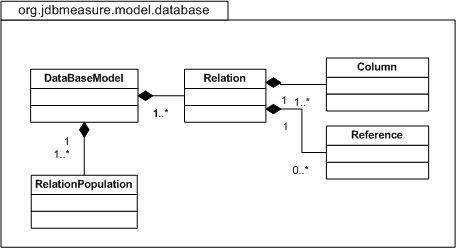
\includegraphics[width=0.8\linewidth]{figures/uml02.png}
\end{center}
\caption{Diagram klas pakietu org.jdbmeasure.model.database}\label{rys:uml02}
\end{figure}
\item org.jdbmeasure.model.load -- dla modelu obciążenia,
\begin{figure}[h]
\begin{center}
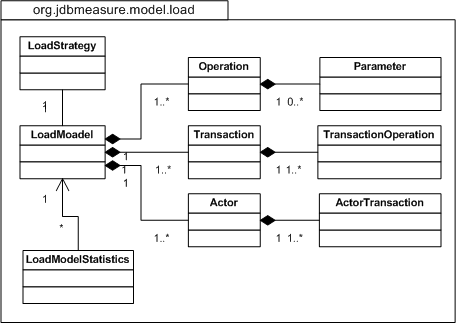
\includegraphics[width=0.8\linewidth]{figures/uml03.png}
\end{center}
\caption{Diagram klas pakietu org.jdbmeasure.model.load}\label{rys:uml03}
\end{figure}
\item org.jdbmeasure.model.test -- dla modelu testu.

\begin{figure}[h]
\begin{center}
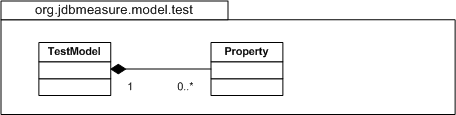
\includegraphics[width=0.8\linewidth]{figures/uml04.png}
\end{center}
\caption{Diagram klas pakietu org.jdbmeasure.model.test}\label{rys:uml04}
\end{figure}

\end{itemize} 

\subsection{Pakiet org.jdbmeasure.rte}
Pakiet org.jdbmeasure.rte zawiera główne klasy klienta RTE. Najważniejsze z nich to:
\begin{itemize}
\item RteClient -- klasa ta implementuje interfejs IRteClient. Jest to interfejs udostępniany poprzez RMI serwerowi benchmarku.
Interfejs IRteClient służy do komunikacji pomiędzy serwerem, a klientem RTE. W związku z tym klasa RteClient jest klasą implementującą
interfejs komunikacyjny z serwerem.
\item ScriptExecutor -- klasa ta służy do wykonywania skryptów testowych.
\item SignalMonitor -- jest to klasa służąca do przekazywania sygnałów synchronizujących pomiędzy klientem RTE a serwerem.
\item RteBeanInfo -- klasa ta dostarcza informacji o środowisku uruchomieniowym klienta RTE. Informacje te dotyczą głównie
ścieżek do katalogów bibliotek, plików wejściowych i wyjściowych, a także sterownika JDBC.
\end{itemize}
Na~rys.~\ref{rys:uml05} przedstawiono diagram klas pakietu org.jdbmeasure.rte.
\begin{figure}[h]
\begin{center}
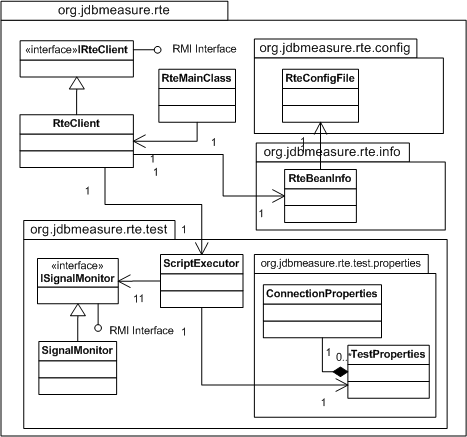
\includegraphics[width=0.8\linewidth]{figures/uml05.png}
\end{center}
\caption{Diagram klas pakietu org.jdbmeasure.rte}\label{rys:uml05}
\end{figure}

\subsection{Pakiet org.jdbmeasure.server}
Pakiet ten zawiera główne klasy serwera benchmarku, a także klasę aplikacji konsolowej (ServerMainClass).
Na~rys.~\ref{rys:uml06} przedstawiono diagram klas tego pakietu. Na uwagę zasługuje interfejs IBenchmarkServer,
jest to interfejs udostępniany klientom RTE poprzez protokół RMI . Klienci wykorzystują go w procesie komunikacji
z serwerem benchmarku. Klasa BenchmarkServer jest implementacją tego interfejsu. Dostarcza ona mechanizmy komunikacji
klient--serwer na wszystkich jej etapach począwszy od połączenia i rejestracji, poprzez deploye'owanie testów,
a skończywszy na przeprowadzaniu procedury testowej i zbieraniu wyników pomiarów.
\begin{figure}[h]
\begin{center}
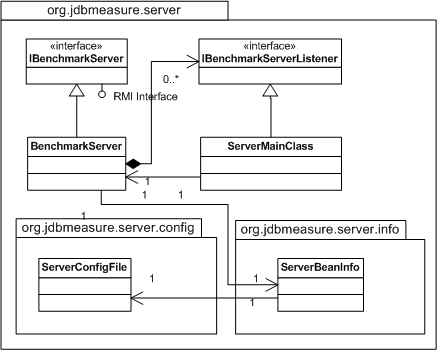
\includegraphics[width=0.8\linewidth]{figures/uml06.png}
\end{center}
\caption{Diagram klas pakietu org.jdbmeasure.server}\label{rys:uml06}
\end{figure}

\subsection{Pakiet org.jdbmeasure.test}
Pakiet ten skupia klasy związane z tworzeniem skryptów testowych, oraz analizą wyników testów (zob.~rys.~\ref{rys:uml07}).
Główną klasą jest tutaj klasa Test, jest ona fasadą dla całego pakietu -- komunikacja z innymi klasami odbywa się bezpośrednio
przez nią. W pakiecie tym możemy wyróżnić trzy podpakiety:
\begin{itemize}
\item org.jdbmeasure.test.datasource -- pakiet klas źródła danych dla klienta RTE, podczas procedury testu.
\item org.jdbmeasure.test.testresult -- pakiet klas reprezentujących przeanalizowany rezultat testu.
\item org.jdbmeasure.test.script -- pakiet klas odpowiedzialnych za generowanie poszczególnych operacji i 
przechowywania metadanych skryptów testowych.
\end{itemize}
\begin{figure}[h]
\begin{center}
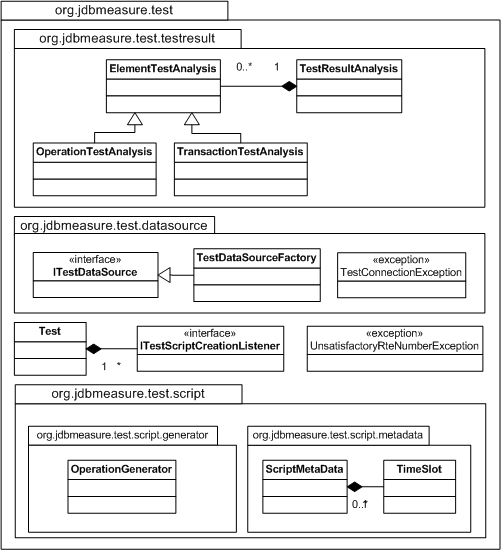
\includegraphics[width=0.8\linewidth]{figures/uml07.png}
\end{center}
\caption{Diagram klas pakietu org.jdbmeasure.test}\label{rys:uml07}
\end{figure}

\subsection{Pakiet org.jdbmeasure.util}
Na pakiet ten składa się grupa niepowiązanych klas, które można określić mianem klas pomocniczych. Do pakietu tego 
należą klasy takie jak:
\begin{itemize}
\item JarClassLoader -- klasa ułatwiająca ładowanie klas z wybranej biblioteki jar.
\item JavaCompiler -- klasa automatyzująca proces kompilacji klas ze wskazanych katalogów, z wykorzystaniem wskazanych bibliotek.
\item FileUtil -- klasa obudowująca podstawowe operacje na plikach i katalogach.
\item FreePortFinder -- klasa ułatwiająca znalezienie wolnego portu.
\item MathExp, MathUtil -- klasy ułatwiające korzystanie z typów BigInteger oraz BigDecimal, a także dostarczające szeregu użytecznych funkcji matematycznych.
\end{itemize}

W bieżącym punkcie zostały omówione główne pakiety projektu JDBMeasure, bliższe informacje 
odnośnie, każdej z klas można znaleźć w dokumentacji JavaDoc.

\section{JDBMeasureRCP - omówienie projektu}
Projekt JDBMeasureRCP jest projektem aplikacji graficznego serwera benchmarku. Jest to aplikacja 
zgodna z modelem Eclipse RCP. Poniżej zamieszczono strukturę pakietów tego projektu. 
\begin{quote}
\begin{Verbatim}
\---org
    \---jdbmeasure
        \---rcp
            +---action -- akcje
            +---bean -- klasy dostosowujące klasy z projektu JDBmeasure 
            +---dialog -- klasy okien dialogowych
            +---editor -- klasy edytorów
            |   +---common
            |   +---databasemodel -- klasy edytora modelu bazy danych
            |   |   +---dialog
            |   |   \---editorpart
            |   +---loadmodel -- klasy edytora modelu obciążenia
            |   |   +---dialog
            |   |   \---editorpart
            |   \---testmodel -- klasy edytora modelu testu
            |       \---editorpart
            +---view -- klasy widoków drzewa i listy podłączonych rte
            +---wizard -- klasy kreatora projektu testu
            \---xmleditor -- klasy edytora xml
\end{Verbatim}
\end{quote}
Projekt ten korzysta z bibliotek zawartych w projekcie JDBMeasureRCPExtJars, który został utworzony
eclipsowym kreatorem ,,Plugin from existing JAR archives''. Do stworzenia wersji gotowej do rozpowszechniania,
należy posłużyć się produktem JDBMeasure.product, wykonując dla niego polecenie ,,Eclipse product export wizard''.

\section{Podsumowanie}
Niniejszy rozdział stanowi opis techniczny benchmarku. Uzupełnieniem tego opisu może być dokumentacja JavaDoc,
dostępna w katalogu /doc/javadoc projektu JDBMeasure. Autor aplikacji dołożył wszelkich starań by w przyszłości
aplikacja była łatwa w rozwoju. W przypadku pytań/problemów służy również swoją pomocą.
